\documentclass[9pt,letterpaper]{extarticle}
\usepackage[T1]{fontenc}
\usepackage{charter}
\usepackage[scaled=0.92]{helvet}
\usepackage[margin=0.45in,top=0.4in,bottom=0.4in]{geometry}
\usepackage{microtype}
\linespread{1.02}
\usepackage{graphicx}
\usepackage{booktabs,tabularx,array}
\usepackage{multicol}
\usepackage[dvipsnames]{xcolor}
\usepackage{enumitem}
\usepackage[hidelinks]{hyperref}

\definecolor{navy}{HTML}{1F3864}
\definecolor{rule}{HTML}{9AA8C0}
\definecolor{pos}{HTML}{1E6B35}
\definecolor{neg}{HTML}{A61B1B}
\pagestyle{empty}
\setlength{\parindent}{0pt}
\setlength{\parskip}{3pt}
\setlength{\columnsep}{14pt}
\setlength{\columnseprule}{0.3pt}
\renewcommand{\columnseprulecolor}{\color{rule}}
\setlist{nosep,leftmargin=1.1em,topsep=2pt,itemsep=1.5pt}
\renewcommand{\arraystretch}{1.15}
\setlength{\tabcolsep}{3.2pt}

\newcommand{\sect}[1]{\par\vspace{7pt}{\sffamily\bfseries\color{navy}\small #1\par}\vspace{1.5pt}{\color{rule}\hrule height 0.4pt}\vspace{3pt}}
\newcommand{\up}[1]{\textcolor{pos}{#1}}
\newcommand{\dn}[1]{\textcolor{neg}{#1}}
\newcommand{\src}[1]{\textsuperscript{\,#1}}

\begin{document}

% ---------------- Header
{\sffamily
\begin{tabularx}{\textwidth}{@{}X r@{}}
{\LARGE\bfseries\color{navy} Long Fabrinet (NYSE: FN)} & {\small Owen Student Fund \textbar{} Youssef Nassar \textbar{} Sep 29, 2026}\\[1pt]
{\large Under-earning long: the capacity bottleneck clears in FY27} 
\end{tabularx}}
\vspace{2pt}

{\sffamily\small
\setlength{\tabcolsep}{0pt}
\begin{tabularx}{\textwidth}{@{}*{6}{>{\centering\arraybackslash}X}@{}}
\toprule
Price (Sep 28) & Target & Bull / Bear & Market cap & Street FY28 EPS & Our FY28 EPS\\
\textbf{\$409.96} & \textbf{\$515 (\up{+26\%})} & \textbf{\$721 / \$265} & \textbf{\$14.7B} & \textbf{\$21.79} & \textbf{\$24.44 (\up{+12\%})}\\
\bottomrule
\end{tabularx}}

\vspace{4pt}
\colorbox{navy!7}{\parbox{\dimexpr\textwidth-2\fboxsep}{\small
Long Fabrinet as an under-earning long. The stock is down 45\% from its high because the market read one quarter of thin margin and negative cash flow as the top of the optics cycle. We think growth was capped by factory space and component supply, and both caps lift this fiscal year as Building~10 completes in early 2027 and laser makers add capacity. The street's numbers imply 5.7\% quarterly growth; we model 8\%, giving FY28 EPS of \$24.44 vs.\ \$21.79, a probability-weighted target of \$515 (+26\%), and 2.1$\times$ more upside in the bull case than downside in the bear.}}

\vspace{2pt}
\begin{multicols}{2}
\small

% ---------------- 1. Overview
\sect{1\quad Business overview}
Contract manufacturer for precision optics: aligns lasers to fiber and photonic chips for transceivers, telecom and data-center links. FY26 (Jul~2025--Jun~2026) revenue \$4.64B (+36\%), non-GAAP EPS \$14.09 (+39\%), net margin $\approx$11\%. Gross margin is thin but steady (12.0\% GAAP), so \emph{earnings move with revenue}. Customers $\geq$10\%: Cisco 20\%, Nvidia 16\% (27.6\% in FY25), Nokia 11\%, Amazon 11\%.\src{1,2} \$875M cash and investments, no debt.\src{1} CEO: Seamus Grady.

% ---------------- 2. Consensus
\sect{2\quad Consensus view}
\textbf{Sellside:} 9 analysts, 7 Buy / 2 Hold, average target \$734. FY27 revenue \$6.10B, EPS \$18.20; FY28 \$7.31B, \$21.79.\src{3} With FQ1 guided to \$1.40B, FY27 implies only \textbf{5.7\% growth per quarter}, and FY28 only 4.0\%, below the 7--16\% FY26 ran at while supply-constrained.

\textbf{Buyside:} the stock fell 19.4\% the day after an FQ4 beat (Aug 18, \$598.58 to \$482.59), on FCF of $-$\$37M from \$92M capex, a slightly slower guide (43\% vs.\ 45\% YoY) and a sector rotation.\src{4,5} At 22.5$\times$ FY27 EPS, the price implies $\approx$27\% year-1 growth fading to 3\% (reverse DCF, 11\% discount rate): roughly street FY27, and \emph{no credit} for new capacity.

% ---------------- 3. Variant
\sect{3\quad Variant view: a supply-side step, not a demand bet}
\begin{enumerate}[label=\arabic*.]
\item \textbf{Demand exceeds shipments.} FQ3 datacom fell 6\% q/q on laser, memory and ASIC shortages; in August management still said component demand exceeds supply, and that the gap is in guidance.\src{5,6}
\item \textbf{The supply is being funded.} Nvidia put \$2B each into Lumentum and Coherent (Mar 2026) with purchase commitments; Lumentum is building a new fab.\src{7}
\item \textbf{Space arrives.} Building~10 (2M sq ft) completes early 2027, adding \$3.0--3.5B capacity to a \$5.3B run rate.\src{2}
\item \textbf{Programs fill it.} Hyperscaler-direct ramp now, merchant program in the Dec quarter, more in early 2027.\src{2}
\item \textbf{Guidance is conservative.} Revenue beat the top of guidance three quarters running (+1.2\% to +3.0\%).\src{1,8}
\end{enumerate}

\begin{tabularx}{\columnwidth}{@{}X rrr@{}}
\toprule
Revenue (\$M) & FQ2 FY26 & FQ3 FY26 & FQ4 FY26\\
\midrule
Actual & 1{,}133 & 1{,}214 & 1{,}316\\
Guide (top) & 1{,}100 & 1{,}200 & 1{,}290\\
Growth q/q \;/\; YoY & 15.8\,/\,35.9\% & 7.2\,/\,39.3\% & 8.4\,/\,44.6\%\\
\bottomrule
\end{tabularx}

\vspace{2pt}
\begin{tabularx}{\columnwidth}{@{}X rr r@{}}
\toprule
& Street & Ours & Gap\\
\midrule
FQ1 FY27 revenue (\$M) & 1{,}400 & 1{,}430 & +2\%\\
q/q growth, FQ2--FQ4 FY27 & 5.7\% & 8.5, 8.5, 8.0\% & +2.6pp\\
FY27 revenue / EPS & \$6.10B / \$18.20 & \$6.48B / \$19.25 & +6\%\\
FY28 revenue / EPS & \$7.31B / \$21.79 & \$8.23B / \$24.44 & +12\%\\
\bottomrule
\end{tabularx}
{\footnotesize Our FQ1 assumes half the recent average beat. FY28: 5\%/quarter, 10.8\% net margin (street 10.9\%); exit run rate \$8.8B, inside Building~10 capacity of \$8.5--9.3B.}

\columnbreak

% ---------------- 4. Risks
\sect{4\quad Key risks and how we would know}
\begin{tabularx}{\columnwidth}{@{}>{\raggedright\arraybackslash}p{0.30\columnwidth} >{\raggedright\arraybackslash}X@{}}
\toprule
Risk & Signal \;$\to$\; action\\
\midrule
AI capex pause & Hyperscaler capex cuts; FQ2 guide $<$ \$1.45B \;$\to$\; exit\\
CPO without FN & Nvidia's Spectrum-X CPO chain (TSMC, SPIL, Lumentum, TFC, Foxconn) omits FN;\src{9} CPO $>$35\% of AI optics by 2030\src{10} \;$\to$\; halve if 2027 attach jumps. Mgmt: near-packaged optics is the nearer opportunity\src{2}\\
Customer shift & A 10\% customer drops (Nvidia went 27.6\% $\to$ 16\% while FN grew 36\%) \;$\to$\; re-underwrite\\
Supply stays tight & Datacom flat q/q again \;$\to$\; hold small\\
Thailand / tariffs & Plant or tariff shock \;$\to$\; size for the tail\\
\bottomrule
\end{tabularx}

\textbf{Kill criteria (written before entry):} two quarters below 5\% q/q growth once Building~10 is qualified; FQ2 guide midpoint below \$1{,}450M; close below \$330 with no news; Building~10 slips past mid-2027.

% ---------------- 5. Risk / reward
\sect{5\quad Risk/reward}
\begin{tabularx}{\columnwidth}{@{}X rrrrr@{}}
\toprule
Case & Prob. & FY28 rev. & EPS & P/E & Value\\
\midrule
Bull: fast fill, CPO win & 25\% & \$9.0B & \$27.72 & 26$\times$ & \$721 \up{(+76\%)}\\
Base: our model & 50\% & \$8.2B & \$24.44 & 22$\times$ & \$538 \up{(+31\%)}\\
Bear: capex pause & 25\% & \$6.3B & \$17.67 & 15$\times$ & \$265 \dn{($-$35\%)}\\
\midrule
\textbf{Probability-weighted} & & & & & \textbf{\$515 \up{(+26\%)}}\\
\bottomrule
\end{tabularx}
{\footnotesize Multiples: 26$\times$ = 5-yr median forward P/E; 22$\times$ = today's; 15$\times$ $\approx$ pre-AI. Net margins 11.2 / 10.8 / 10.2\%.}

\textbf{Breakeven:} the bear case must exceed \textbf{60\%} probability before expected value falls to today's price.

\vspace{1pt}
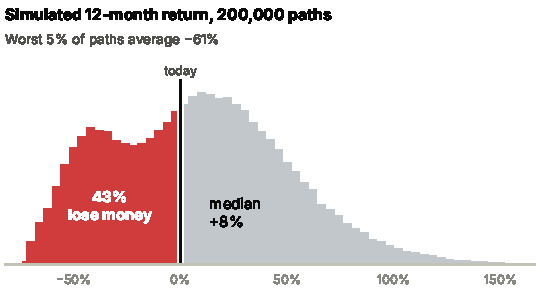
\includegraphics[width=\columnwidth]{mc_returns.pdf}
{\footnotesize Revenue sets both earnings and the multiple, which is what fattens the left tail.}

\textbf{Sizing:} realized volatility 85\% (50 days, incl.\ earnings gap), 49\% (20 days). Full Kelly $\approx$0.43; we size at $\approx$5\%, adding toward 10\% if FQ1 confirms — the worst-5\% case then costs the fund $\approx$2.6\%.

% ---------------- 6. Signposts
\sect{6\quad Catalysts and signposts}
\begin{itemize}
\item \textbf{Early Nov 2026:} Lumentum FQ1 (laser supply read-through), then FN FQ1: revenue $\geq$ \$1{,}430M, FQ2 guide midpoint $\geq$ \$1{,}500M.
\item \textbf{Early 2027:} Building~10 completion; FQ2 (Feb) growth near 8\% q/q.
\item \textbf{Rolling:} sellside FY28 EPS moving from \$21.79 toward \$24; FN named in any CPO supply chain; datacom q/q; insider selling.
\end{itemize}

\end{multicols}

\vspace{-4pt}
{\color{rule}\hrule height 0.4pt}
\vspace{2pt}
{\scriptsize\color{black!70}
\textbf{Sources} (Sep 29, 2026): [1] FN 8-K releases FQ1--FQ4 FY26, SEC EDGAR. [2] FN FQ4 FY26 earnings call, Aug 17, 2026. [3] S\&P Global consensus via StockAnalysis.com, Sep 23, 2026. [4] FN daily prices, StockAnalysis.com. [5] FQ4 reaction coverage, TIKR. [6] FQ3 FY26 call summary. [7] optics.org, Mar 3, 2026. [8] Guidance in each prior 8-K. [9] StorageReview, Aug 15, 2026. [10] TrendForce via I/O Fund. Reverse DCF, scenarios and Monte Carlo: author's model (FN\_Thesis\_Tracker.xlsx, montecarlo.py). Fiscal year ends late June. Educational use in a student fund; not investment advice.\par}

\end{document}